\section{Pattern Classification on Non Linearly Separable Data}

\subsection{K-Nearest Neighbours Classifier}

The given synthetic data is classified using KNN Method. The training data is of the shape of a spiral with 3 arcs corresponding to each class. Let us look at some interesting plots obtained for the KNN method for the given dataset. 

The dip in accuracy of the models in training, validation and test dataset is because of the ambiguity at the end of each arc of the spiral as well as at the centre of it. Otherwise the model seems to classify other data points well and the decision plots give a good representation of them. For \textit{K=7} we get a 100$\%$ prediction in both test and validation data. We represent the decision plots for different values of K.

\hspace{5cm}
% -----------------------------------------------------------
{\rowcolors{3}{green!40!yellow!10}{green!0!yellow!30}
\begin{table}[!h]
\centering
\begin{tabular}{ |c|c|c|  }
\hline
\rowcolor{lightgray} Model & Training Accuracy & Val Accuracy\\
\hline
K=1 & 99.84$\%$  & 100$\%$  \\   
 \hline
K=7 & 99.50$\%$  & 100$\%$  \\ 
 \hline
K=15 & 99.67$\%$  & 100$\%$ \\ 
\hline
\end{tabular}
\caption{Performance of various KNN Models}.
\label{table:3}
\end{table}
}

\newpage

%------------------------------------------------------------
\subsubsection{Plots for K=1}

\begin{figure}[!ht]
    \centering
    \begin{subfigure}[t]{0.5\textwidth}
        \centering
        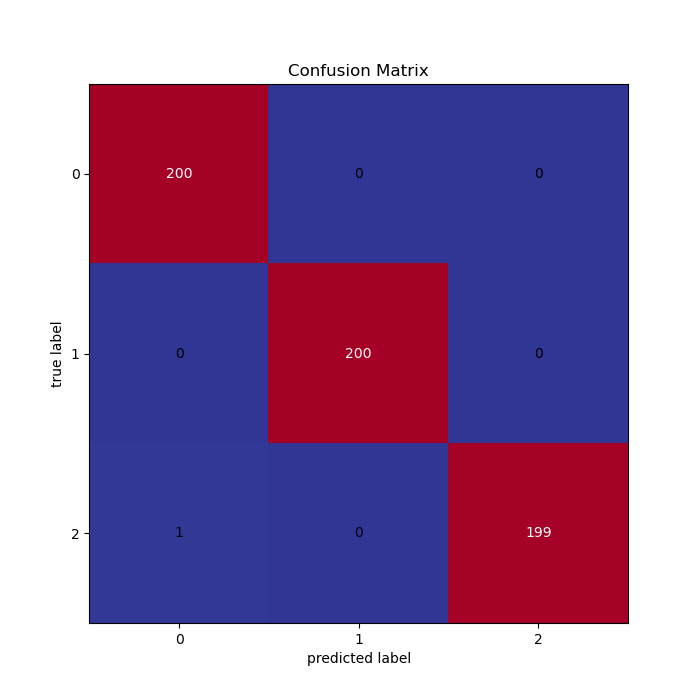
\includegraphics[height=2.5in]{Dataset_1b/K_1_cmatrix_train_data.png}
        \caption{Confusion Matrix for training data}
    \end{subfigure}%
    ~ 
    \begin{subfigure}[t]{0.5\textwidth}
        \centering
        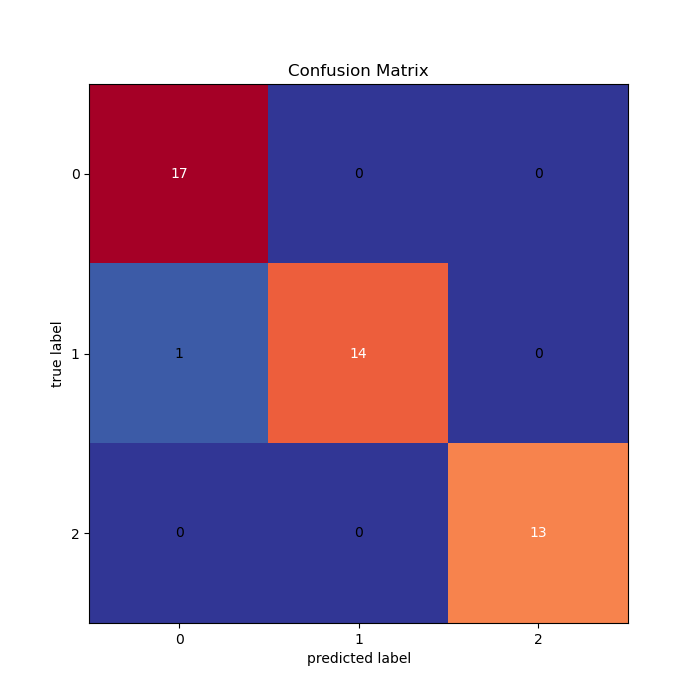
\includegraphics[height=2.5in]{Dataset_1b/K_1_cmatrix_test_data.png}
        \caption{Confusion Matrix for test data}
    \end{subfigure}%
    ~
    \caption{Confusion Matrix for KNN Model trained with K=1}
    \label{fig:13}
\end{figure}

% -----------------------------------------------------------
\begin{figure}[!ht]
    \centering
    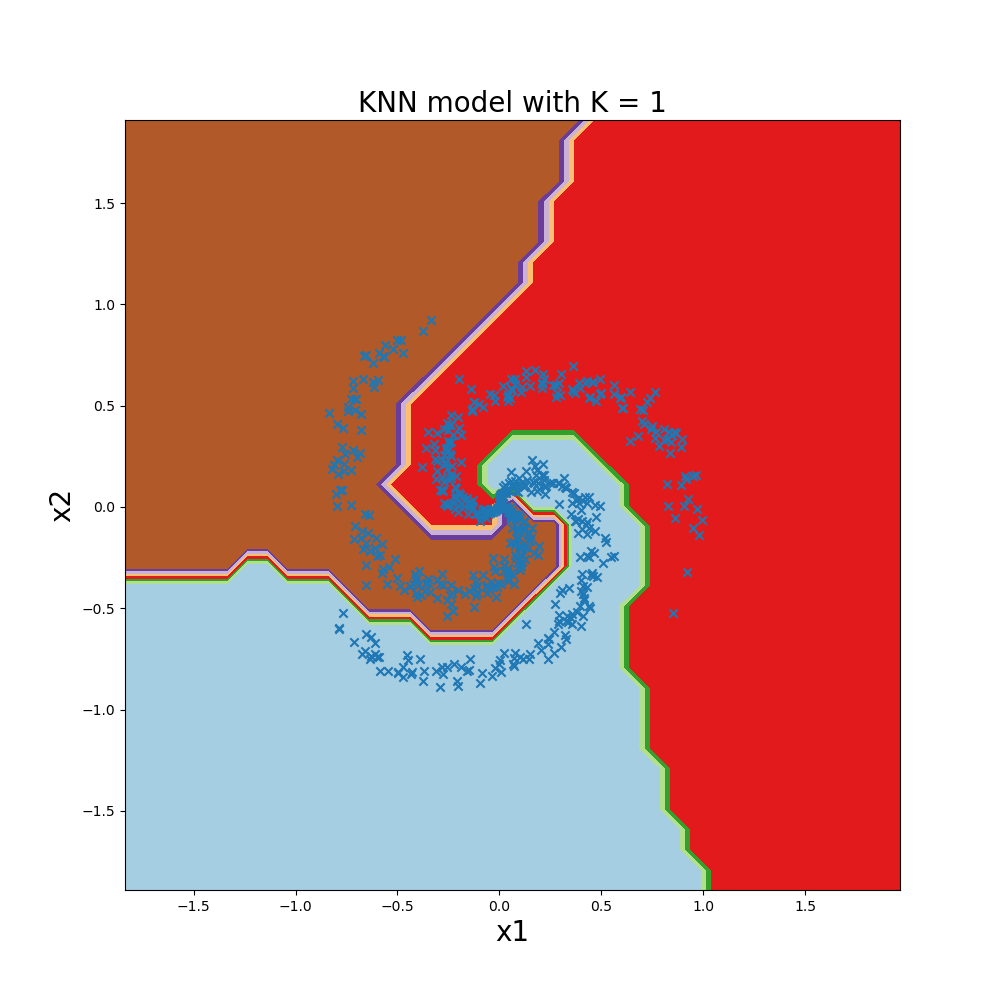
\includegraphics[height=3.5in]{Dataset_1b/K_1_decision_plot.png}
    \caption{Decision Plot KNN Model trained with K=1}
    \label{fig:14}
\end{figure}

\newpage
% -----------------------------------------------------------
\subsubsection{Plots for K=7}

\begin{figure}[!ht]
    \centering
    \begin{subfigure}[t]{0.5\textwidth}
        \centering
        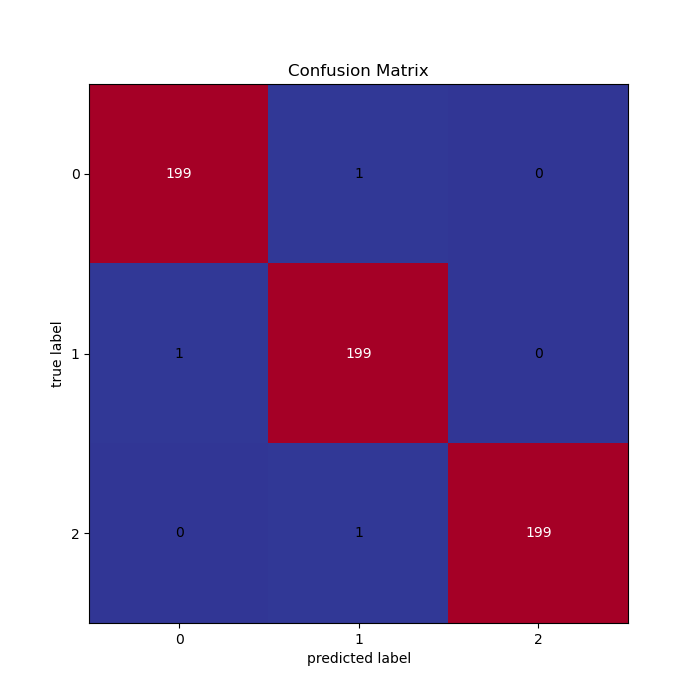
\includegraphics[height=2.5in]{Dataset_1b/K_7_cmatrix_train_data.png}
        \caption{Confusion Matrix for training data}
    \end{subfigure}%
    ~ 
    \begin{subfigure}[t]{0.5\textwidth}
        \centering
        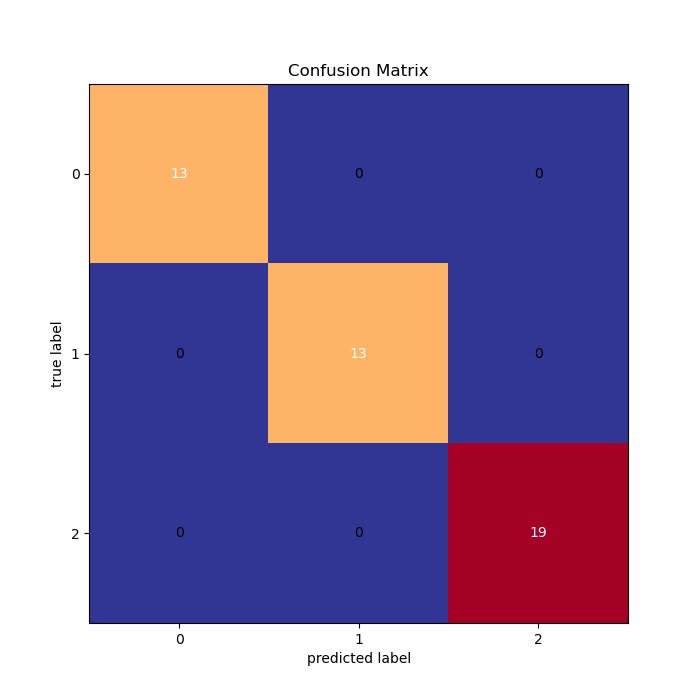
\includegraphics[height=2.5in]{Dataset_1b/K_7_cmatrix_test_data.png}
        \caption{Confusion Matrix for test data}
    \end{subfigure}%
    ~
    \caption{Confusion Matrix for KNN Model trained with K=7}
    \label{fig:15}
\end{figure}
% -----------------------------------------------------------
\begin{figure}[!ht]
    \centering
    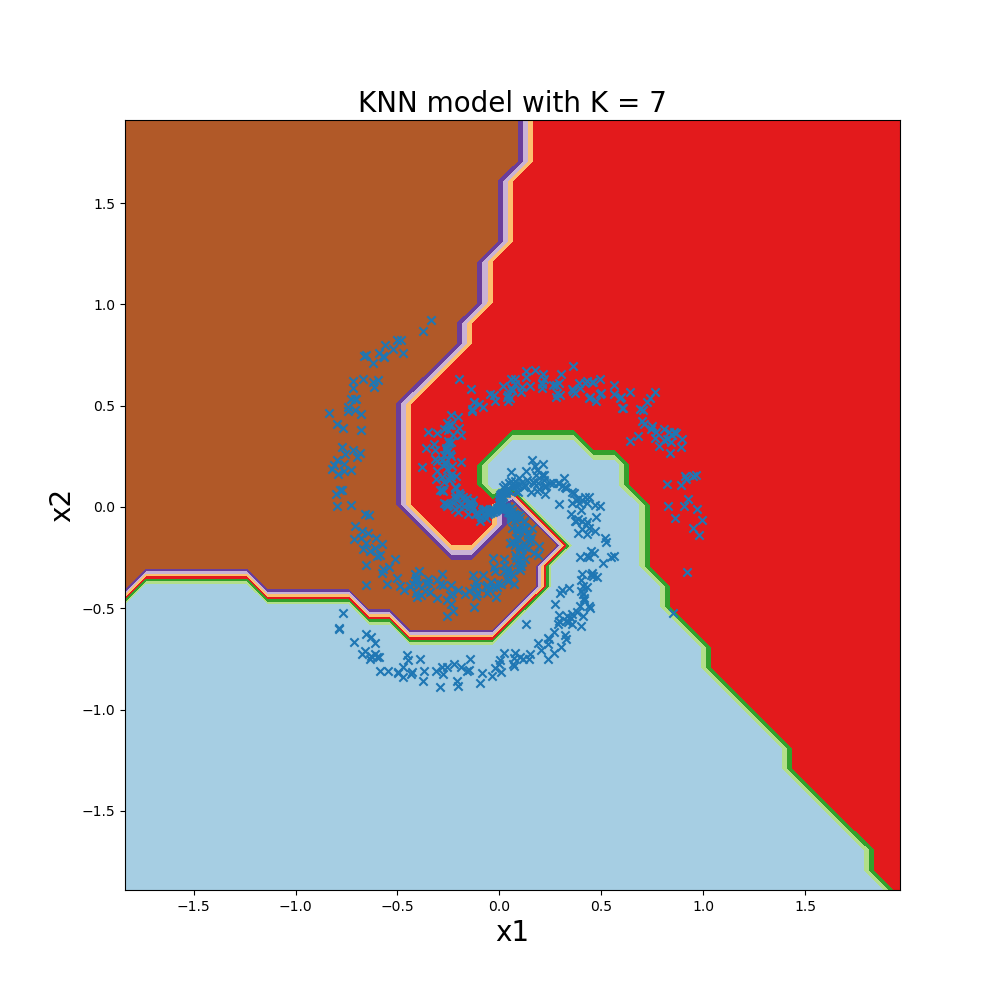
\includegraphics[height=3.5in]{Dataset_1b/K_7_decision_plot.png}
    \caption{Decision Plot KNN Model trained with K=7}
    \label{fig:16}
\end{figure}

\newpage
% -----------------------------------------------------------
\subsubsection{Plots for K=15}

\begin{figure}[!ht]
    \centering
    \begin{subfigure}[t]{0.5\textwidth}
        \centering
        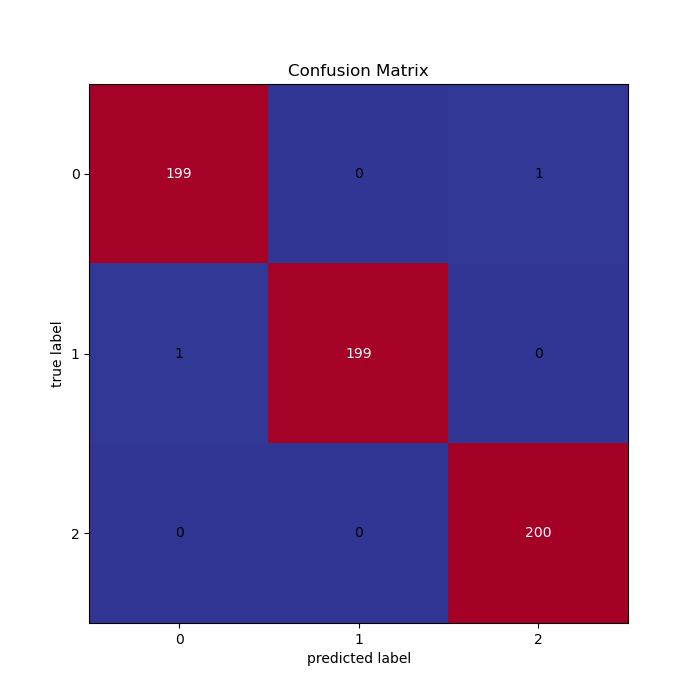
\includegraphics[height=2.5in]{Dataset_1b/K_15_cmatrix_train_data.png}
        \caption{Confusion Matrix for training data}
    \end{subfigure}%
    ~ 
    \begin{subfigure}[t]{0.5\textwidth}
        \centering
        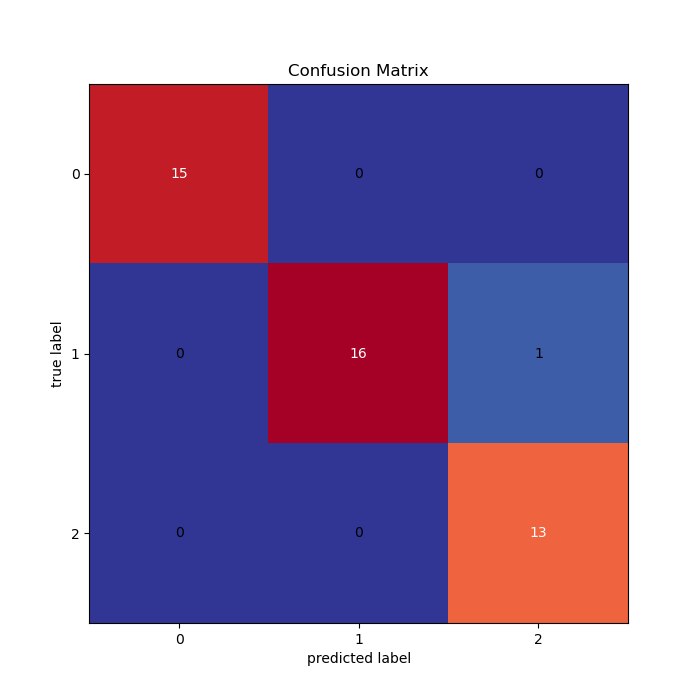
\includegraphics[height=2.5in]{Dataset_1b/K_15_cmatrix_test_data.png}
        \caption{Confusion Matrix for test data}
    \end{subfigure}%
    ~
    \caption{Confusion Matrix for KNN Model trained with K=15}
    \label{fig:17}
\end{figure}
% -----------------------------------------------------------
\begin{figure}[!ht]
    \centering
    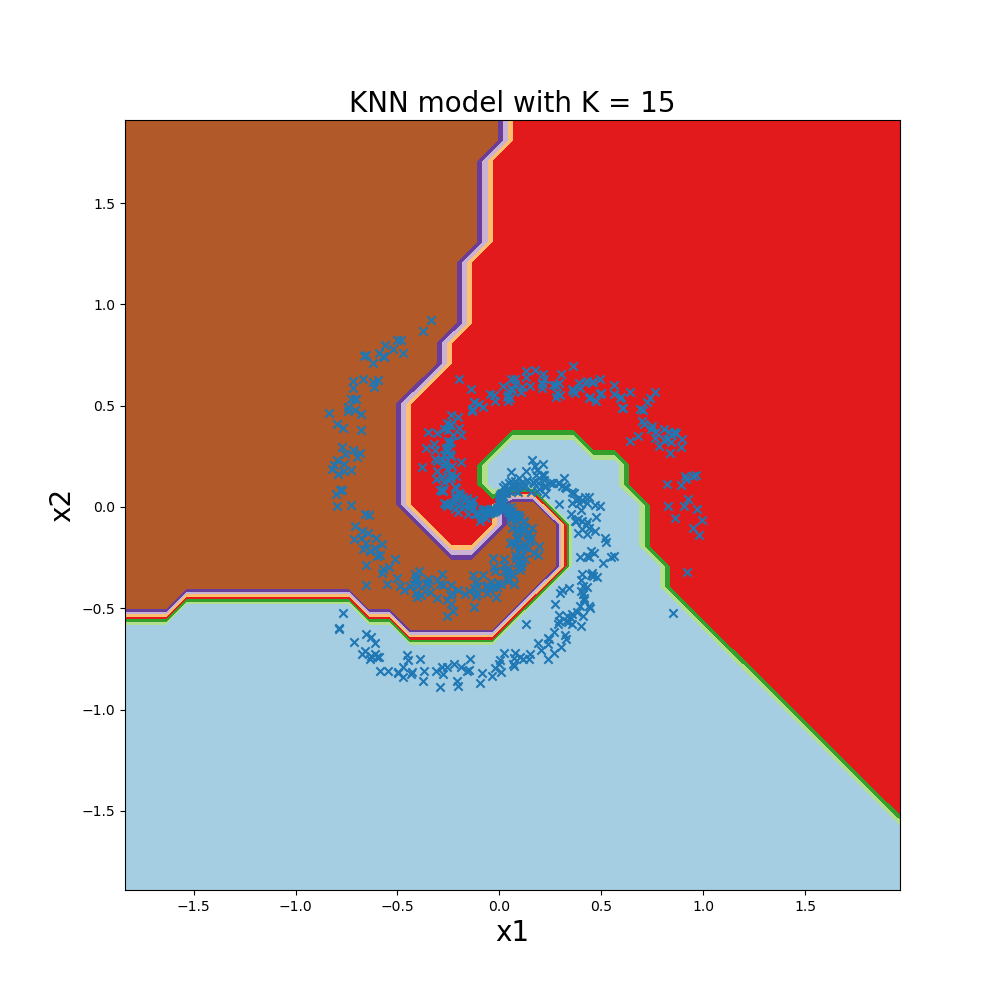
\includegraphics[height=3.5in]{Dataset_1b/K_15_decision_plot.png}
    \caption{Decision Plot KNN Model trained with K=15}
    \label{fig:18}
\end{figure}

\newpage
%------------------------------------------------------------
\subsection{Bayes Classifier with GMM and diagonal covariance matrix}

In this method we represent the density function of a class with weighted normal distributions each trying to capture the non-linearity in the system. Let us look at interesting results for different hyper parameters which in this case is the number of normal functions used.

% -----------------------------------------------------------

{\rowcolors{3}{green!40!yellow!10}{green!0!yellow!30}
\begin{table}[!h]
\centering
\begin{tabular}{ |c|c|c| }
\hline
\rowcolor{lightgray} Model & Training Accuracy & Val Accuracy\\
\hline
[1,1,1] & 52.17$\%$  & 60$\%$ \\   
 \hline
[3,3,3] & 98.84$\%$  & 100$\%$ \\ 
\hline
[5,5,5] & 98.84$\%$  & 100$\%$ \\ 
\hline
[7,7,7] & 98.84$\%$  & 100$\%$ \\ 
\hline
[10,10,10] & 98.84$\%$  & 100$\%$\\ 
\hline
[15,15,15] & 99.67$\%$  & 100$\%$ \\ 
\hline
\end{tabular}
\caption{Performance of various Models}.
\label{table:4}
\end{table}
}

In the above table [x,y,z] represents the corresponding number of normal distributions in each class. In our case there are a total of 3 classes. Based on the above table, we can see that the accuracy increases as we increase the number of normal distributions. This means that the non-linearities in each class will now be modelled by more functions and thus the increase in accuracy. Similar to KNN, it has trouble modelling data near the centre of the spiral as well as at the end which accounts for the dip in accuracy in certain cases. We will generalize that our [7,7,7] model to be the good one in this case since it performs slightly better in the val and test set with 100$\%$ accuracy in both of them. Other models even though there is a 100$\%$ validation accuracy, there was a slight dip in performance in the test set. Let us look at the confusion matrix and decision plot corresponding to that model. \\

From \ref{fig:20}, since we use a diagonal covariance matrix, the level curves of the normal distribution assumed are parallel to the XY axes. The decision region modelled is also completely non linear which shows the power of this particular model as compared to others

\begin{figure}[!ht]
    \centering
    \begin{subfigure}[t]{0.5\textwidth}
        \centering
        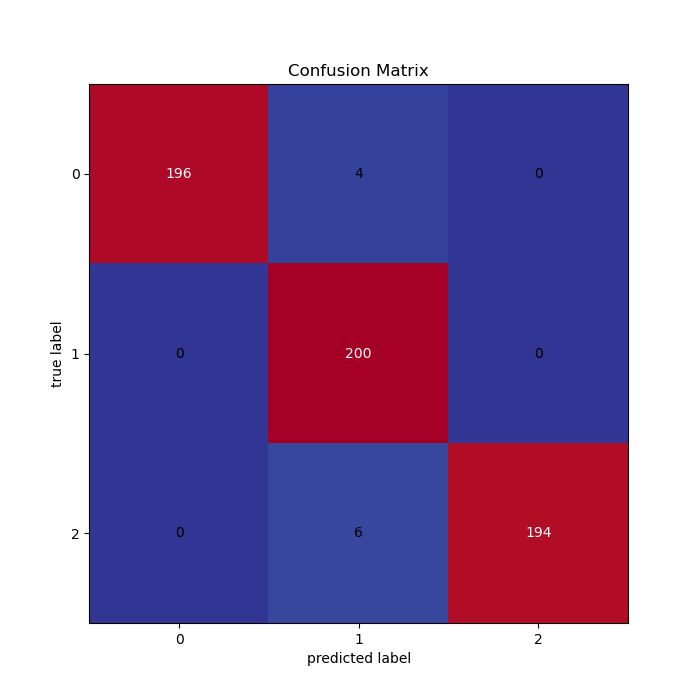
\includegraphics[height=2.5in]{Dataset_1b/GMM_7_cmatrix_train_data_diag.png}
        \caption{Confusion Matrix for training data}
    \end{subfigure}%
    ~ 
    \begin{subfigure}[t]{0.5\textwidth}
        \centering
        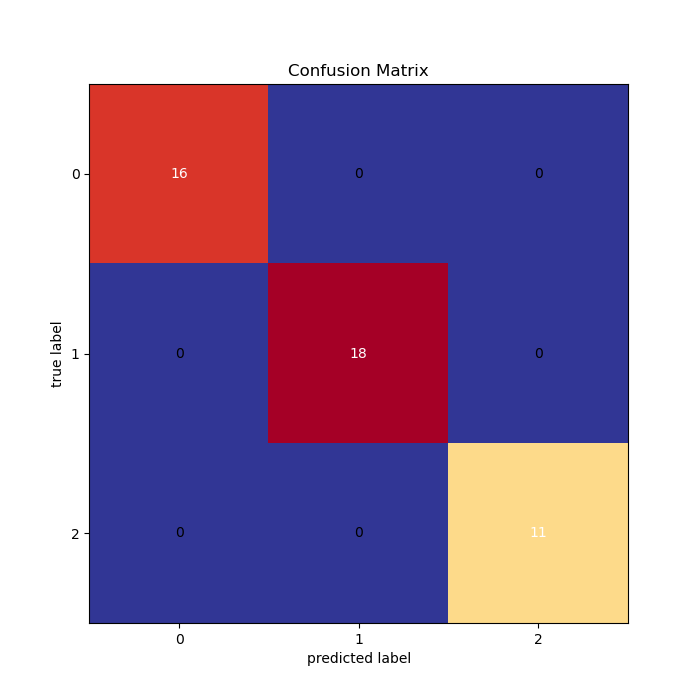
\includegraphics[height=2.5in]{Dataset_1b/GMM_7_cmatrix_test_data_diag.png}
        \caption{Confusion Matrix for test data}
    \end{subfigure}%
    ~
    \caption{Confusion Matrix for GMM model with diagonal covariance matrix}
    \label{fig:19}
\end{figure}

% -----------------------------------------------------------
\begin{figure}[!ht]
    \centering
    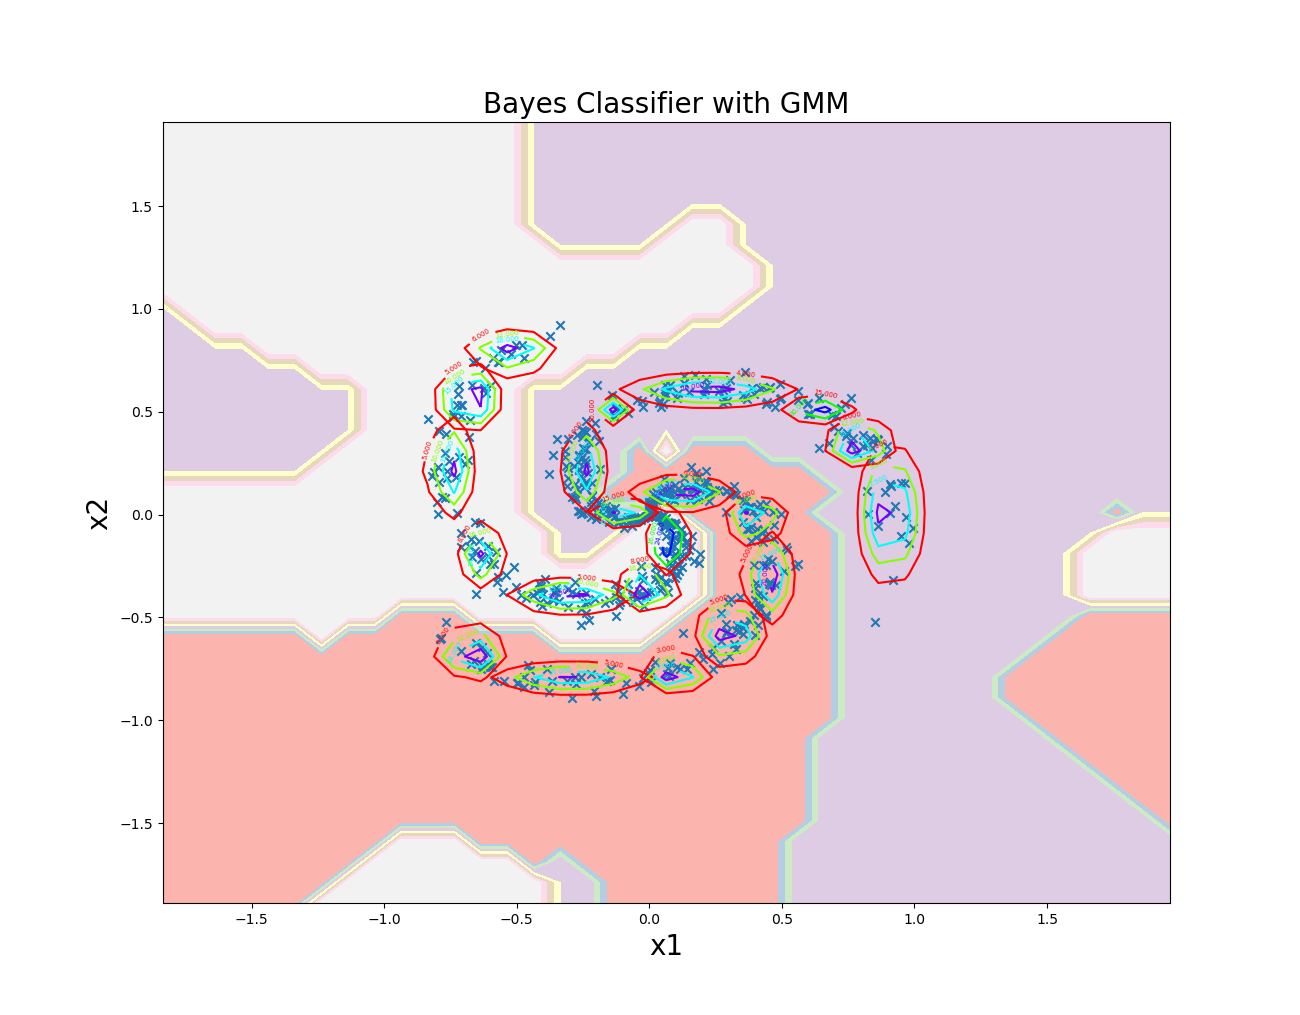
\includegraphics[height=3.5in]{Dataset_1b/GMM_7_decision_plot_diag.png}
    \caption{Decision Plot of GMM model with diagonal covariance matrix}
    \label{fig:20}
\end{figure}


\newpage
%------------------------------------------------------------
\subsection{Bayes Classifier with GMM and full covariance matrix}

In this method we represent the density function of a class with weighted normal distributions each trying to capture the non-linearity in the system. Let us look at interesting results for different hyper parameters which in this case is the number of normal functions used.

% -----------------------------------------------------------

{\rowcolors{3}{green!40!yellow!10}{green!0!yellow!30}
\begin{table}[!h]
\centering
\begin{tabular}{ |c|c|c|  }
\hline
\rowcolor{lightgray} Model & Training Accuracy & Val Accuracy \\
\hline
[1,1,1] & 59.17$\%$  & 66.67$\%$\\   
 \hline
[3,3,3] & 98.84$\%$  & 100$\%$ \\ 
\hline
[5,5,5] & 99.67$\%$  & 100$\%$\\ 
\hline
[7,7,7] & 99.67$\%$  & 100$\%$ \\ 
\hline
[10,10,10] & 99.67$\%$  & 100$\%$  \\ 
\hline
[15,15,15] & 99.67$\%$  & 100$\%$  \\ 
\hline
\end{tabular}
\caption{Performance of various Models}.
\label{table:5}
\end{table}
}

In the above table [x,y,z] represents the corresponding number of normal distributions in each class. In our case there are a total of 3 classes. Based on the above table, we can see that the accuracy increases as we increase the number of normal distributions. This means that the non-linearities in each class will now be modelled by more functions and thus the increase in accuracy. Similar to KNN, it has trouble modelling data near the centre of the spiral as well as at the end which accounts for the dip in accuracy in certain cases. We will generalize that our [10,10,10] model to be the good one in this case since it performs slightly better in the val and test set. Let us look at the confusion matrix and decision plot corresponding to that model. \\

As shown in \ref{fig:22}, since we use a full covariance matrix, the level curves of the normal distribution is different than the previous case and now is oriented in a different way. This would mean more number of parameter estimations but better modelling of non linearities. The decision region modelled is also completely non-linear and seems to have a higher non-linearity as compared to the case with diagonal covariance matrix which shows the power of this particular model as compared to others

\begin{figure}[!ht]
    \centering
    \begin{subfigure}[t]{0.5\textwidth}
        \centering
        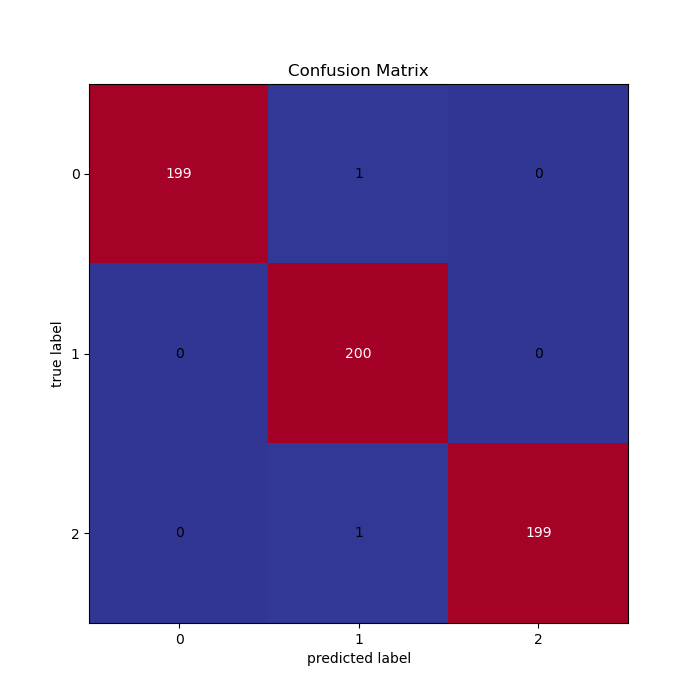
\includegraphics[height=2.5in]{Dataset_1b/GMM_10_cmatrix_train_data_non_diag.png}
        \caption{Confusion Matrix for training data}
    \end{subfigure}%
    ~ 
    \begin{subfigure}[t]{0.5\textwidth}
        \centering
        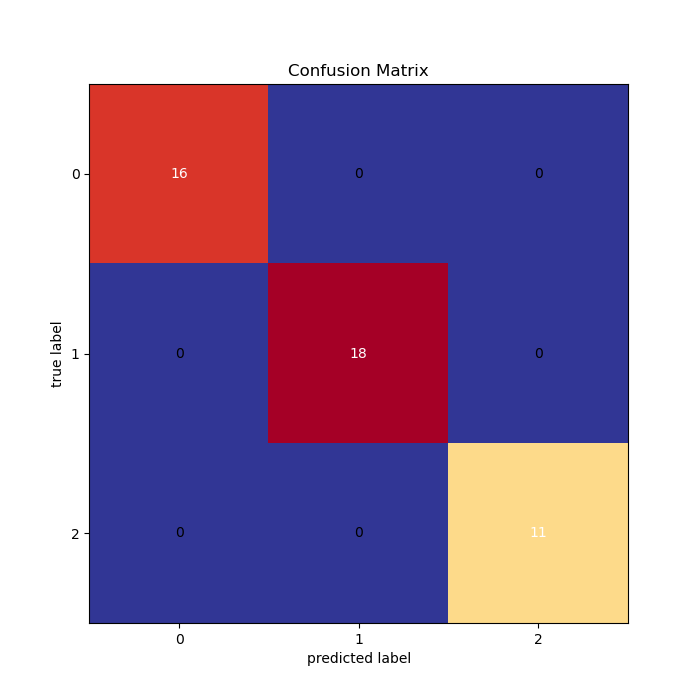
\includegraphics[height=2.5in]{Dataset_1b/GMM_10_cmatrix_test_data_non_diag.png}
        \caption{Confusion Matrix for test data}
    \end{subfigure}%
    
    \caption{Confusion Matrix for GMM model with full covariance matrix}
    \label{fig:21}
\end{figure}

% -----------------------------------------------------------
\begin{figure}[!ht]
    \centering
    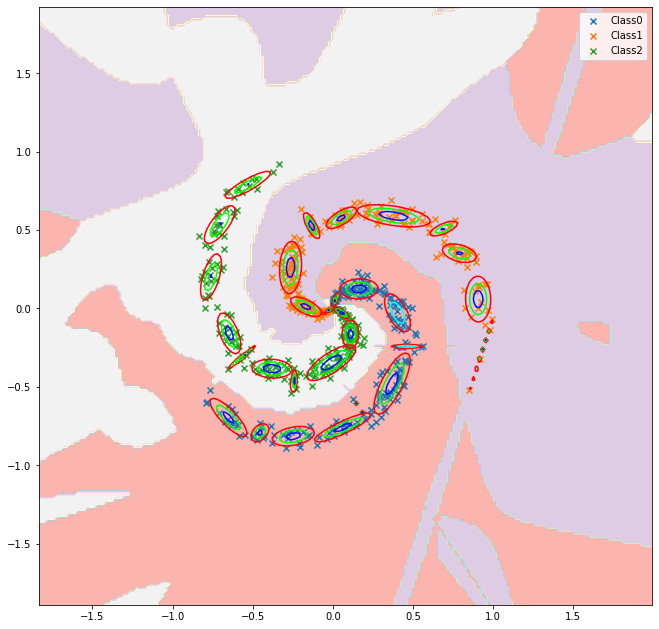
\includegraphics[height=3.5in]{Dataset_1b/GMM_10_decision_plot_non_diag.png}
    \caption{Decision Plot of GMM model with full covariance matrix}
    \label{fig:22}
\end{figure}

%------------------------------------------------------------
\newpage
\subsection{Bayes Classifier with KNN Density Estimation}
In this method we represent the density function in a different way as explained in the initial sections. Let us look at some interesting plots.

The dip in the accuracy is similar to what was observed in the KNN method. The problem occurs in the end of the arc of the spiral and the centre of it where the method is ambiguous in determining the nearest neighbours in an effective way similar to other models we have seen. The test accuracy was 97.78$\%$ in both the cases. The decision surfaces of both the models are plotted. As we increase the value of \textit{K} we see that the decision boundary fails to cature the end of the spiral of each clas. This may be because, we may now have more data points in the other class which may possibly make the decision boundary move towards them.

\hspace{5cm}
% -----------------------------------------------------------
{\rowcolors{3}{green!40!yellow!10}{green!0!yellow!30}
\begin{table}[!h]
\centering
\begin{tabular}{ |c|c|c|  }
\hline
\rowcolor{lightgray} Model & Training Accuracy & Val Accuracy \\
\hline
K=10 & 99.67$\%$  & 100$\%$ \\   
 \hline
K=20 & 98.67$\%$  & 100$\%$ \\ 
\hline
\end{tabular}
\caption{Performance of various Models}.
\label{table:6}
\end{table}
}

\newpage
%------------------------------------------------------------
\subsubsection{Plots for K=10}

\begin{figure}[!ht]
    \centering
    \begin{subfigure}[t]{0.5\textwidth}
        \centering
        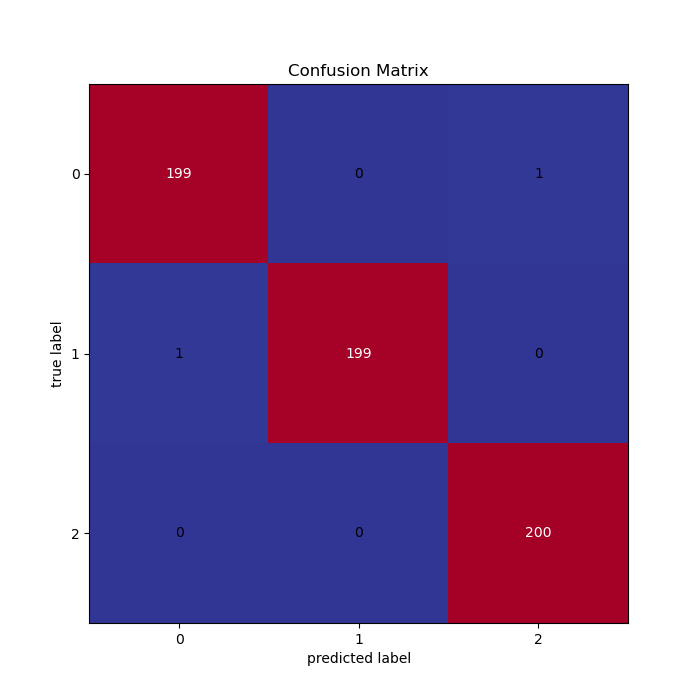
\includegraphics[height=2.5in]{Dataset_1b/K_10_cmatrix_train_data_bayes.png}
        \caption{Confusion Matrix for training data}
    \end{subfigure}%
    ~ 
    \begin{subfigure}[t]{0.5\textwidth}
        \centering
        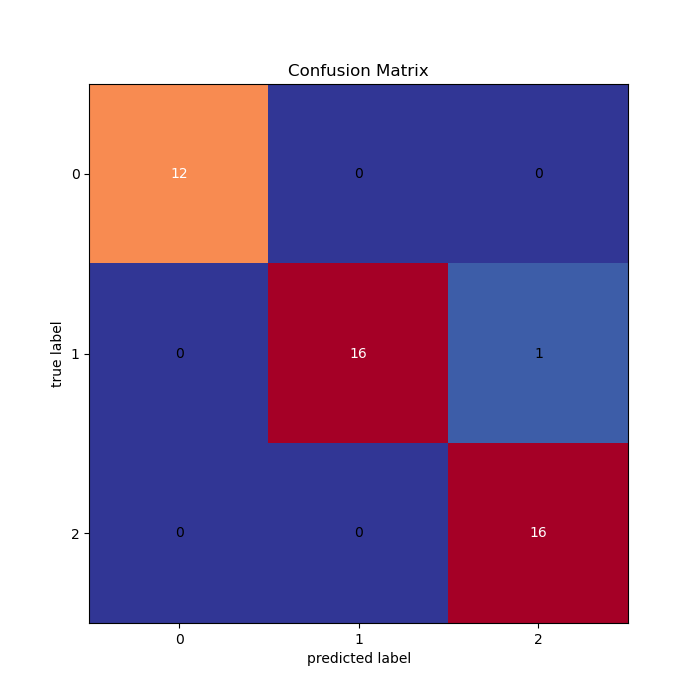
\includegraphics[height=2.5in]{Dataset_1b/K_10_cmatrix_test_data_bayes.png}
        \caption{Confusion Matrix for test data}
    \end{subfigure}%
    ~
    \caption{Confusion Matrix with K=10}
    \label{fig:23}
\end{figure}

% -----------------------------------------------------------
\begin{figure}[!ht]
    \centering
    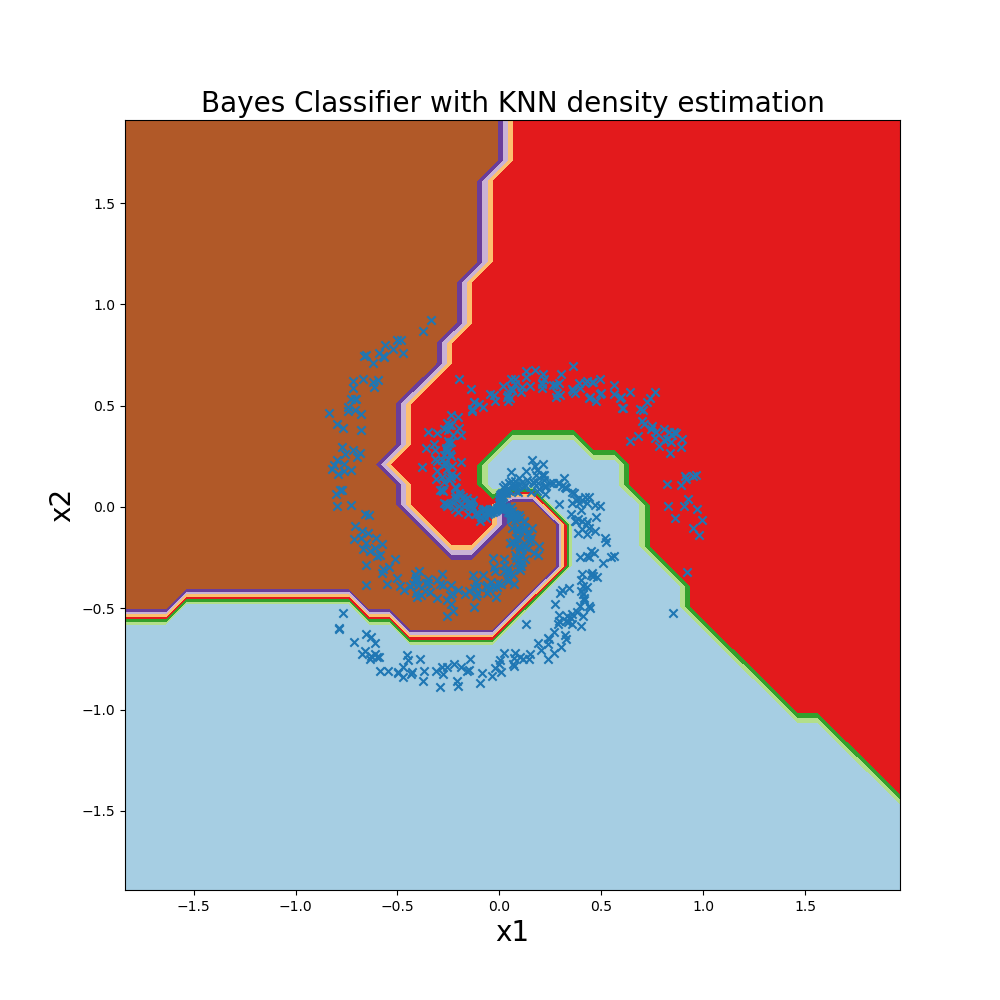
\includegraphics[height=3.5in]{Dataset_1b/K_10_decision_plot_bayes.png}
\     \caption{Decision Plot with K=1}
    \label{fig:24}
\end{figure}
\newpage
% -----------------------------------------------------------
\subsubsection{Plots for K=20}

\begin{figure}[!ht]
    \centering
    \begin{subfigure}[t]{0.5\textwidth}
        \centering
        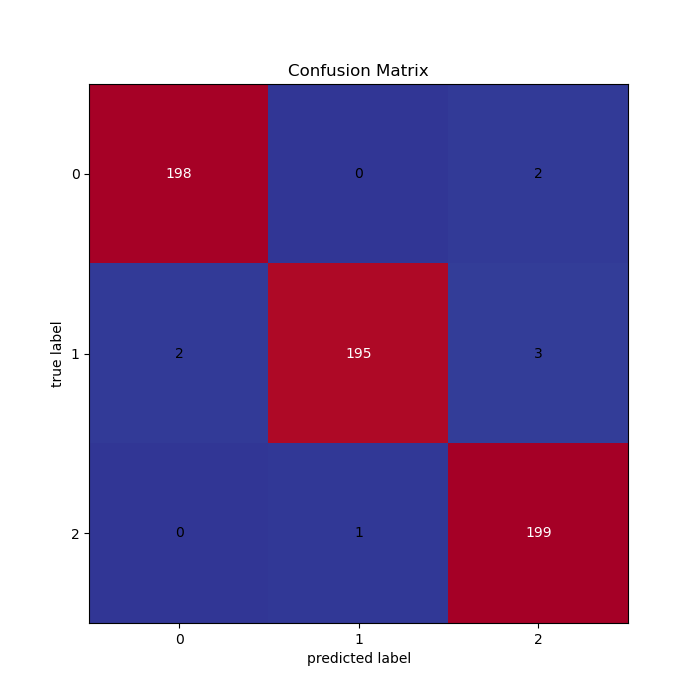
\includegraphics[height=2.5in]{Dataset_1b/K_20_cmatrix_train_data_bayes.png}
        \caption{Confusion Matrix for training data}
    \end{subfigure}%
    ~ 
    \begin{subfigure}[t]{0.5\textwidth}
        \centering
        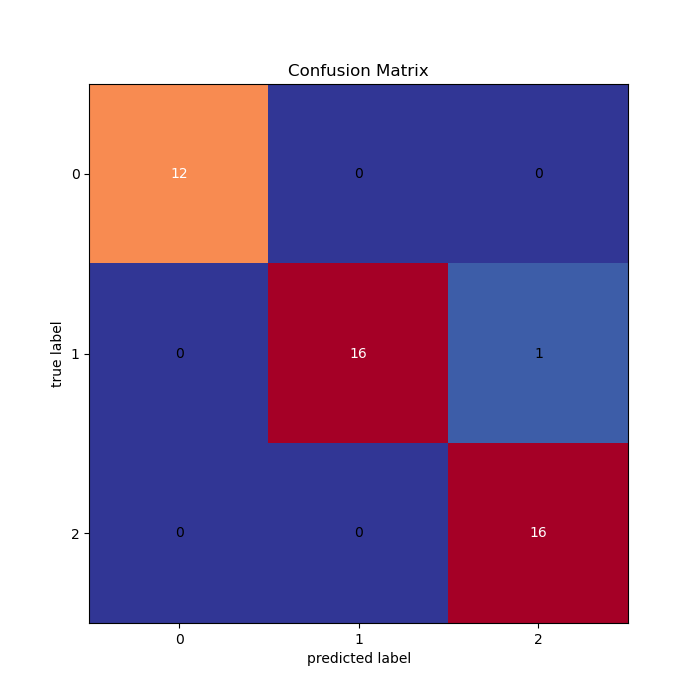
\includegraphics[height=2.5in]{Dataset_1b/K_20_cmatrix_test_data_bayes.png}
        \caption{Confusion Matrix for test data}
    \end{subfigure}%
    ~
    \caption{Confusion Matrix with K=20}
    \label{fig:25}
\end{figure}
% -----------------------------------------------------------
\begin{figure}[!ht]
    \centering
    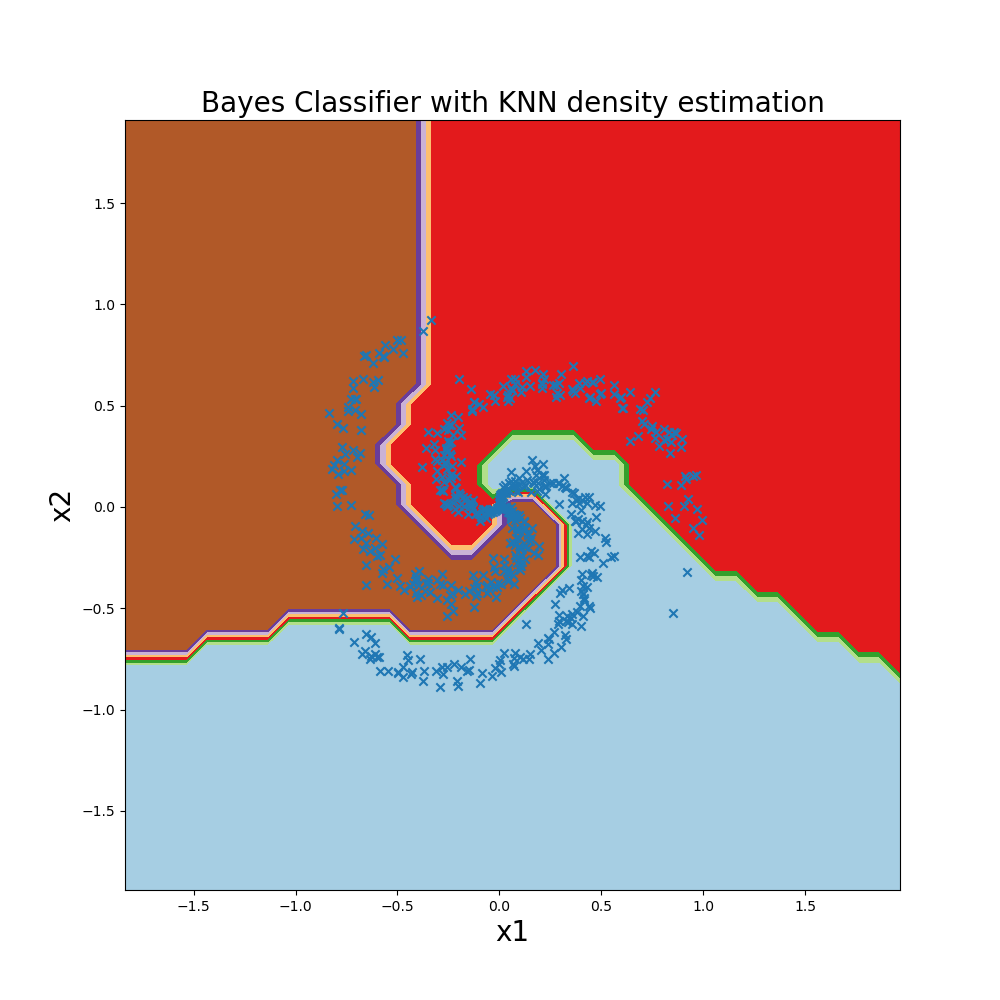
\includegraphics[height=3.5in]{Dataset_1b/K_20_decision_plot_bayes.png}
    \caption{Decision Plot with K=20}
    \label{fig:26}
\end{figure}
